\documentclass{beamer}
\usepackage[utf8]{inputenc}

\usetheme{Madrid}
\usecolortheme{default}
\usepackage{amsmath}
\usepackage{amssymb,amsfonts,amsthm}
\usepackage{txfonts}
\usepackage{tkz-euclide}
\usepackage{listings}
\usepackage{adjustbox}
\usepackage{array}
\usepackage{tabularx}
\usepackage{gvv}
\usepackage{lmodern}
\usepackage{circuitikz}
\usepackage{tikz}
\usepackage{graphicx}

\setbeamertemplate{page number in head/foot}[totalframenumber]

\usepackage{tcolorbox}
\tcbuselibrary{minted,breakable,xparse,skins}

\definecolor{bg}{gray}{0.95}
\DeclareTCBListing{mintedbox}{O{}m!O{}}{%
  breakable=true,
  listing engine=minted,
  listing only,
  minted language=#2,
  minted style=default,
  minted options={%
    linenos,
    gobble=0,
    breaklines=true,
    breakafter=,,,
    fontsize=\small,
    numbersep=8pt,
    #1},
  boxsep=0pt,
  left skip=0pt,
  right skip=0pt,
  left=25pt,
  right=0pt,
  top=3pt,
  bottom=3pt,
  arc=5pt,
  leftrule=0pt,
  rightrule=0pt,
  bottomrule=2pt,
  toprule=2pt,
  colback=bg,
  colframe=orange!70,
  enhanced,
  overlay={%
    \begin{tcbclipinterior}
    \fill[orange!20!white] (frame.south west) rectangle ([xshift=20pt]frame.north west);
    \end{tcbclipinterior}},
  #3,
}
\lstset{
    language=C,
    basicstyle=\ttfamily\small,
    keywordstyle=\color{blue},
    stringstyle=\color{orange},
    commentstyle=\color{green!60!black},
    numbers=left,
    numberstyle=\tiny\color{gray},
    breaklines=true,
    showstringspaces=false,
}

\title{1.9.14}
\date{29th August, 2025}
\author{AI25btech11014-Suhas}

\begin{document}

\frame{\titlepage}

\begin{frame}{Question}
The centroid of triangle $\triangle ABC$ is at $\vec{G} = \myvec{1\\1\\1}$.  
Given:  
$\vec{A} = \myvec{3\\-5\\7}$,  
$\vec{B} = \myvec{-1\\7\\-6}$  
Find: Coordinates of point $\vec{C}$.
\end{frame}

\begin{frame}{Theoretical Solution}
Centroid formula:  
\begin{align}
\vec{G} = \frac{1}{3}(\vec{A} + \vec{B} + \vec{C})
\end{align}
Multiply both sides by 3:  
\begin{align}
3\vec{G} = \vec{A} + \vec{B} + \vec{C}
\end{align}
Rearranged:  
\begin{align}
\vec{C} = 3\vec{G} - \vec{A} - \vec{B}
\end{align}
\end{frame}

\begin{frame}{Theoretical Solution}
Let $\vec{A} = \vec{a}$, $\vec{B} = \vec{b}$, $\vec{G} = \vec{g}$  
Then:  
\begin{align}
\vec{C} = 3\vec{g} - \vec{a} - \vec{b}
\end{align}
Numerical substitution:  
\begin{align}
\vec{C} = 3\myvec{1\\1\\1} - \myvec{3\\-5\\7} - \myvec{-1\\7\\-6}
\end{align}
\end{frame}

\begin{frame}{Theoretical Solution}
Step-by-step:  
\begin{align}
3\vec{G} = \myvec{3\\3\\3} \\
\vec{C} = \myvec{3\\3\\3} - \myvec{3\\-5\\7} = \myvec{0\\8\\-4} \\
\vec{C} = \myvec{0\\8\\-4} - \myvec{-1\\7\\-6} = \myvec{1\\1\\2}
\end{align}
Answer:  
$\vec{C} = \myvec{1\\1\\2}$
\end{frame}

\begin{frame}[fragile]
\frametitle{C Code - Direct Solve}
\begin{lstlisting}
#include <stdio.h>

int main() {
    double A[3] = {3, -5, 7};
    double B[3] = {-1, 7, -6};
    double G[3] = {1, 1, 1};
    double C[3];

    for (int i = 0; i < 3; i++)
        C[i] = 3 * G[i] - A[i] - B[i];

    printf("C = (%lf, %lf, %lf)\n", C[0], C[1], C[2]);
}
\end{lstlisting}
\end{frame}

\begin{frame}[fragile]
\frametitle{C Code - Function for .so}
\begin{lstlisting}
#include <stdio.h>

void centroid(double* A, double* B,
              double* G, double* C) {
    for (int i = 0; i < 3; i++) {
        C[i] = 3 * G[i] - A[i] - B[i];
    }
}
\end{lstlisting}
\end{frame}

\begin{frame}[fragile]
\frametitle{Python Code - Setup}
\begin{lstlisting}
import ctypes
import numpy as np

lib = ctypes.CDLL("./libcentroid.so")
lib.centroid.argtypes = [
    ctypes.POINTER(ctypes.c_double)
] * 4
\end{lstlisting}
\end{frame}

\begin{frame}[fragile]
\frametitle{Python Code - Execution}
\begin{lstlisting}
A = np.array([3.0, -5.0, 7.0])
B = np.array([-1.0, 7.0, -6.0])
G = np.array([1.0, 1.0, 1.0])
C = np.zeros(3)

A_ct = A.ctypes.data_as(
    ctypes.POINTER(ctypes.c_double))
B_ct = B.ctypes.data_as(
    ctypes.POINTER(ctypes.c_double))
\end{lstlisting}
\end{frame}

\begin{frame}[fragile]
\frametitle{Python Code - Result}
\begin{lstlisting}
G_ct = G.ctypes.data_as(
    ctypes.POINTER(ctypes.c_double))
C_ct = C.ctypes.data_as(
    ctypes.POINTER(ctypes.c_double))

lib.centroid(A_ct, B_ct, G_ct, C_ct)

print("Coordinates of C:", C)
\end{lstlisting}
\end{frame}

\begin{frame}{Plot}

\begin{figure}[H]
    \centering
    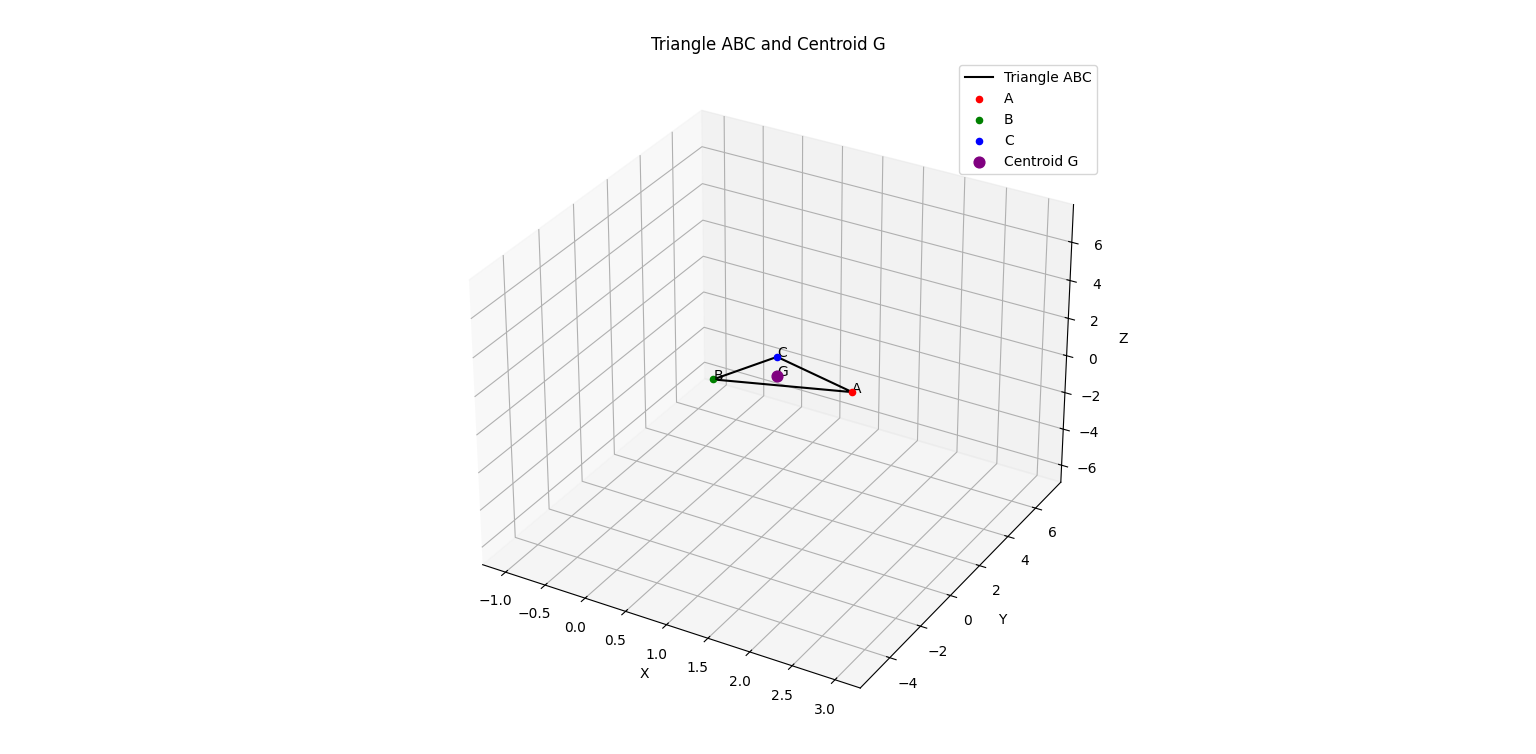
\includegraphics[width=01\textwidth]{figs/fig1.png}
    \caption{Plot}
    \label{Plot}
\end{figure}

\end{frame}






\end{document}